\hypertarget{architecture_intro}{}\section{Introduction}\label{architecture_intro}
Please refer the Main Page for an introduction\hypertarget{architecture_goals}{}\section{Goals}\label{architecture_goals}
The approach to do topic modelling is to have a graphical model representing the generative assumptions the user has about the corpus. A graphical model is a probabilistic model representing the joint distribution of the random variables involved with a graph denoting the conditional independence assumptions amongst them. Solving the model is to infer the parameters of the model by processing the actual data. Doing this inference is the hardest part of the approach.\hypertarget{architecture_new_models}{}\subsection{Adding new Models}\label{architecture_new_models}
There are a lot of variations on the basic LDA model and with each variation the inferencing logic changes. The parameters, the sufficient statistics that need to be maintained everything will be slightly different. One of the main goals of this framework is to make the job of adding new models simpler.\hypertarget{architecture_infrastructure}{}\subsection{Common Infrastructure}\label{architecture_infrastructure}
One task that is mostly common across multiple models is the infrastructure needed to store documents, load them, create a pipeline that can optimally utilize multi-\/core parallelism. In the framework we aim to standardize on proven infrastructure that is known to provide efficient implementations so that the model writer just worries about adding only the parts that are relevant for doing the inference\hypertarget{architecture_scalability}{}\subsection{Scalability}\label{architecture_scalability}
Another main aspect of this framework is to substantially increase the scale of the state of the art by utilizing parallelism both multi-\/core and multi-\/machine.\hypertarget{architecture_components}{}\section{Main components of the System}\label{architecture_components}
Y!LDA uses the Gibbs sampling approach popularized by \href{http://dx.doi.org/10.1073%2Fpnas.0307752101}{\tt Collapsed Gibbs Sampling}. There are four main components in this approach: 
\begin{DoxyEnumerate}
\item {\bfseries \hyperlink{class_model}{Model}:}\par
 This encapsulates the parameters of the model and the sufficient statistics that are necessary for inference 
\item {\bfseries \hyperlink{class_model___refiner}{Model\_\-Refiner}:}\par
 This encapsulates the logic needed for refining the initial model which involves streaming the documents from disk, sampling new topic assignments, updating the model, performing diagnostics and optimization and writing the documents back to disk 
\item {\bfseries \hyperlink{class_pipeline}{Pipeline}:}\par
 As can be seen above, the refiner does a sequence of operations on every document of the corpus. Some of them have to run serially but some others can be run parallely. To enable exploiting multi-\/core parallelism, the \hyperlink{class_pipeline}{Pipeline} is defined to be composed of a set of operations called filters which can either be declared to be run serially or parallely. The \hyperlink{class_pipeline}{Pipeline} comes with a scheduler that schedules the threads available on the machine to run these filters in an optimal fashion 
\item {\bfseries \hyperlink{class_execution___strategy}{Execution\_\-Strategy}:}\par
 This encapsulates the strategy that decides what filters a pipeline is composed of, how many times the documents are passed through the pipeline. 
\end{DoxyEnumerate}\hypertarget{architecture_builder}{}\subsection{Builder Pattern}\label{architecture_builder}
The Builder pattern fits very well for this approach. We implement a \hyperlink{class_model___builder}{Model\_\-Builder} that builds the last three components depending on what model is needed and what mode the model is supposed to operate in.

The \hyperlink{class_model___builder}{Model\_\-Builder} creates an initial \hyperlink{class_model}{Model} and creates the required \hyperlink{class_model___refiner}{Model\_\-Refiner} by passing the Model(or the necessary components of the Model). It then creates a \hyperlink{class_pipeline}{Pipeline} and an \hyperlink{class_execution___strategy}{Execution\_\-Strategy} as per the mode of operation.

The Director is pretty straightforward. It directs the given \hyperlink{class_model___builder}{Model\_\-Builder} to create the necessary components and executes the defined \hyperlink{class_execution___strategy}{Execution\_\-Strategy}. This refines the initial \hyperlink{class_model}{Model} created by the builder into one that reflects parameters tuned to the corpus on which the \hyperlink{class_model}{Model} was refined on. Then the \hyperlink{class_model}{Model} is stored on disk for testing.\hypertarget{architecture_multi-machine}{}\section{Distributed Set Up}\label{architecture_multi-machine}
To cater to the Scalability goals, as detailed in \href{http://portal.acm.org/citation.cfm?id=1920931}{\tt An Architecture for Parallel Topic Models}, the framework implements a Distributed Memory based multi-\/machine setup that exploits multi-\/machine parallelism to the fullest. The main idea being that the inferencing happens locally while the state variables are kept up-\/to-\/date with a global copy that stored using a Distributed HashTable. To come up with an efficient distributed set up is a difficult thing and we definitely do not want people reinvent the wheel here. So the framework tries to abstract the mechanism of distribution, the implementation of an efficient distributed HashTable and the mechanism needed for Synchrnoization.\hypertarget{architecture_distributed_map}{}\subsection{Distributed\_\-Map}\label{architecture_distributed_map}
The framework implements a Distributed\_\-Map interface using Ice as a very efficient middleware. It essentially provides both a Server and \hyperlink{class_client}{Client} implementation. 
\begin{DoxyEnumerate}
\item {\bfseries \hyperlink{class_d_m___server}{DM\_\-Server}:}\par
 The server essentially hosts a chunk of the distributed hash table and supports the usual map operations. It also supports three special operations: 
\begin{DoxyItemize}
\item Put: Which accumulates the values instead of replacing 
\item waitForAll: Which is a barrier implementation using AMD 
\item PutNGet: which is an asynchronous call that accumulates the passed value into the existing one and returns the final value back to the caller through a call back mechanism  
\end{DoxyItemize}
\item {\bfseries \hyperlink{class_d_m___client}{DM\_\-Client}:} \par
 A client that supports a single hash table view of the distributed system. The client transparently supports a rate limited, sliding-\/window based Asynchronous Method Invocation for the PutNGet which is a very useful operation to have for effective Synchronization. Refer to the VLDB paper for more information.  
\end{DoxyEnumerate}

For most models, one need not worry about modifying the above. These only need to be used most of the times without bothering much about their implementation.\hypertarget{architecture_synchronizer}{}\subsection{Synchronizer}\label{architecture_synchronizer}
The framework provides a default implementation of the Synchronization strategy detailed in \mbox{[}2\mbox{]}. The \hyperlink{class_synchronizer}{Synchronizer} is run as a separate background thread apart from the main threads that do the inferencing. The actual task of synchronization is left to the implementation of a \hyperlink{class_synchronizer___helper}{Synchronizer\_\-Helper} class. The Sychronizer only creates slots for synchronization and asks the helper to synchronize in those slots. It also takes care of running the Synchronization only till the inferencing is done.

However, there is a strong assumption that the synchronization proceeds in a linear fashion. That is the structures being synchronized are linear and can be synchronized one after the other. This is implicit in the Synchronizer's creation of slots.\hypertarget{architecture_synchronizer_helper}{}\subsection{Synchronizer\_\-Helper}\label{architecture_synchronizer_helper}
Every model has to only provide the \hyperlink{class_synchronizer___helper}{Synchronizer\_\-Helper} implementation which spills the logic for synchronizing the model's relevant structures, maintains copies of them where needed and provides the callback function for the AMI putNGet.\hypertarget{architecture_default_impl}{}\section{Default Implementations provided}\label{architecture_default_impl}
The framework provides default implementations for the \hyperlink{class_pipeline}{Pipeline} interface and the Execution\_\-Stratgey interface. 
\begin{DoxyEnumerate}
\item {\bfseries \hyperlink{class_t_b_b___pipeline}{TBB\_\-Pipeline}:}\par
 This implementation uses Intel's Threading Building Blocks for providing the \hyperlink{class_pipeline}{Pipeline} interface. 
\item {\bfseries \hyperlink{class_training___execution___strategy}{Training\_\-Execution\_\-Strategy}:}\par
 The default implementation of \hyperlink{class_execution___strategy}{Execution\_\-Strategy} for LDA training. Assembles the following pipeline for data flow:  
\begin{DoxyImageNoCaption}
  \mbox{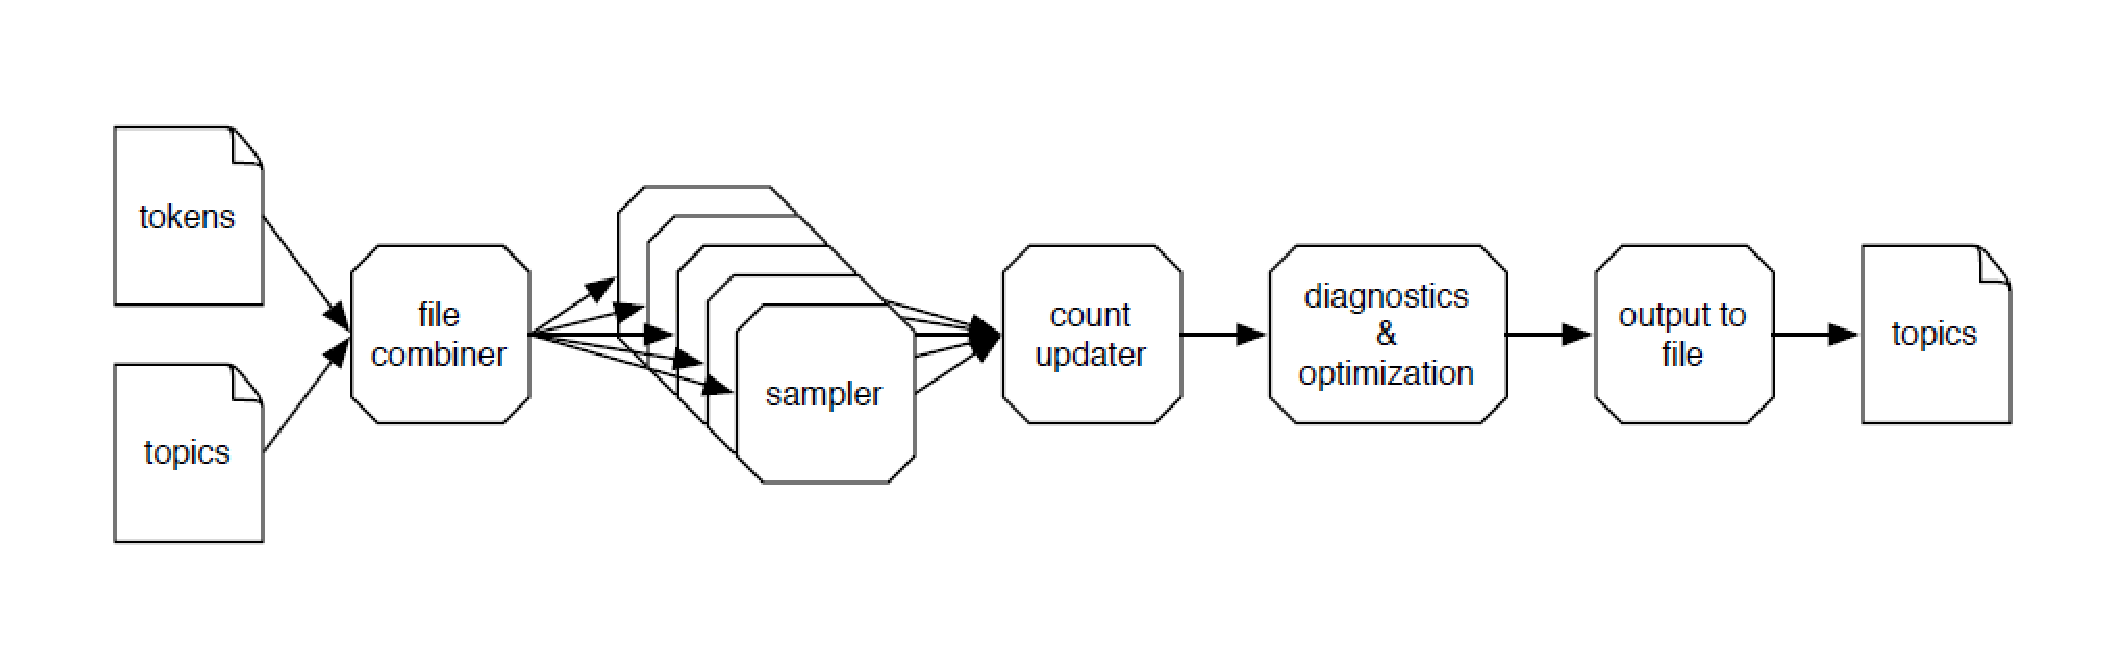
\includegraphics{data_flow}}
\end{DoxyImageNoCaption}
 
\item {\bfseries \hyperlink{class_synchronized___training___execution___strategy}{Synchronized\_\-Training\_\-Execution\_\-Strategy}:}\par
 The default implementation of \hyperlink{class_execution___strategy}{Execution\_\-Strategy} that extends \hyperlink{class_training___execution___strategy}{Training\_\-Execution\_\-Strategy} and adds Synchronization capability 
\item {\bfseries \hyperlink{class_testing___execution___strategy}{Testing\_\-Execution\_\-Strategy}:}\par
 The default implementation of \hyperlink{class_execution___strategy}{Execution\_\-Strategy} for LDA testing.


\end{DoxyEnumerate}\hypertarget{architecture_unigram}{}\section{Unigram Model}\label{architecture_unigram}
The framework also provides the \hyperlink{class_unigram___model}{Unigram\_\-Model} implementations of the various common interfaces. This is the basic LDA model with the bag of words assumption. Please take a look at how the various interfaces are implemented. The main implementation needed is for \hyperlink{class_model}{Model} \& \hyperlink{class_model___refiner}{Model\_\-Refiner}. Additionally, it implements efficient sparse data structures to store the sufficient statistics.\hypertarget{architecture_new_model}{}\section{Adding a new Model}\label{architecture_new_model}
Please use the \hyperlink{class_unigram___model}{Unigram\_\-Model} implementation as an example to implement new models\hypertarget{architecture_chkpt}{}\section{Checkpoints}\label{architecture_chkpt}
The framework also provide checkpointing functionality for the multi-\/machine setup in order to provide failure recovery. This is implemented by an external object that knows how to do three things: a. Serialize metadata to disk b. load previously serialized metadata on request c. Serialize the datastructures to disk

An appropriate checkpointer is passed as an argument while creating an \hyperlink{class_execution___strategy}{Execution\_\-Strategy} The strategy uses checkpointers to checkpoint at regular intervals. At startup, it also checks if any checkpoints are available and if so, it starts up from that checkpoint.

Different checkpointers are needed for different setups. For ex., the framework uses the Local \hyperlink{class_checkpointer}{Checkpointer} when running in single machine mode which only involves writing the iteration number as metadata. All other data needed for restart is already being serialized. However, for the multi-\/machine setup, a different mechanism is needed and a Hadoop \hyperlink{class_checkpointer}{Checkpointer} is implemented.

This is an ongoing effort and we will add more stuff both to the code and documentation. We definitely need your help \& contribution in making this better.

Here is an initial set of TODOs:

\begin{Desc}
\item[\hyperlink{todo__todo000001}{Todo}]Add unit tests to make the code more robust 

Add more code documentation for the \hyperlink{class_unigram___model}{Unigram\_\-Model} components 

Implement fancier models in later versions 

Implement extensions to the LDA model in later versions\end{Desc}
These are in no particular order and we might re-\/prioritize later. Please mail me if you are interested in contributing

We shall use the git pull request (fork + pull model) for collaborative development. 